\documentclass[../main/main.tex]{subfiles}

\raggedbottom

\makeatletter
\renewcommand{\@chapapp}{\'Electrocin\'etique -- chapitre}
\makeatother

\begin{document}
\setcounter{chapter}{3}

\chapter{Oscillateurs harmonique et amorti}

Dans le chapitre précédent, nous avons vu des systèmes qui présentent un régime
transitoire caractérisé par des exponentielles croissantes ou décroissantes. En
combinant deux de ces composants, on trouve alors des régimes transitoires
caractérisé par une combinaison d'exponentielles, exprimée sous la forme de
fonctions sinusoïdales. Regardons un exemple.

\section{Introduction harmonique}

\subsection{Signal sinusoïdal}

\begin{tcbraster}[raster columns=2, raster equal height=rows]
    \begin{defi}[label=def:signsu]{signal sinusoïdal}

        Un signal sinusoïdal est un signal de la forme
        \[ \boxed{s(t) = A\cos(\wt + \f)}\]

        $A$ est l'\textit{amplitude}, telle que
        \[ A = \frac{s_{\max} - s_{\min}}{2}\]

        $\wt +f$ est la \textit{phase instantanée} du signal, avec
        \vspace*{-20pt}
        \begin{center}
            \begin{tikzpicture}[]
                \node[anchor=center] (name) at (0,0)
                    {\textcolor{cornflowerblue}{$\w$}$t$+\textcolor{limegreen}{$\f$}};
                \node[inner sep=0] (datab) at ([shift={(0,3pt)}]name.south west) {};
                \node[inner sep=0] (biasb) at ([shift={(0,3pt)}]name.south east) {};
                \node[below left =.5cm and .5cm of datab, color=cornflowerblue] (data)
                    {pulsation};
                \node[below right=.5cm and .5cm of biasb, color=limegreen] (bias)
                    {phase initiale};
                \draw[-stealth] (data) -- (datab);
                \draw[-stealth] (bias) -- (biasb);
            \end{tikzpicture}
        \end{center}
        \tcbsubtitle[before skip=\baselineskip,
        colback=green!50!black,
        colframe=green!50!black]{Unités}
        La phase s'exprime en \textbf{radians}~; la pulsation en
        \textbf{\si{rad.s^{-1}}}.
    \end{defi}
    \begin{exem}[label=exem:graph]{graphique}
        \begin{center}
            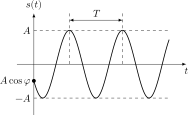
\includegraphics[width=\linewidth]{ch8-fig1}
        \end{center}
        La pulsation représente la vitesse avec de variation de la phase, et
        s'exprime en \si{rad.s^{-1}}. Pour une variation de $2\pi$ effectuée à
        la période $T$, on définit
        \begin{center}
            \fbox{$\w = 2\pi/T = 2\pi f$}
        \end{center}
    \end{exem}
\end{tcbraster}

\subsection{Équation différentielle oscillateur harmonique}

\begin{tcbraster}[raster columns=2, raster equal height=rows]
    \begin{prop}[label=prop:eqdiffoh]{équation différentielle}
        Un oscillateur harmonique à un degré de liberté est un système dont
        l'évolution temporelle est décrite par une grandeur $x(t)$ solution
        d’une équation différentielle du type~:

        \[ \boxed{ \dv[2]{x}{t} + \w_0{}^2x = \w_0{}^2x_{\rm eq}}\]

        Avec $x_{\rm eq}$ la position d'équilibre du système et $\w_0$ la
        pulsation \textbf{propre}.
    \end{prop}
    \begin{prop}[label=prop:soluoh]{solutions}
        La forme générale des solutions d'un oscillateur harmonique s'écrit de
        manière équivalente
        \begin{empheq}[box=\fbox]{gather*}
            x(t) = A'\cos(\w_0 t + \f) + x_{\rm eq}\\
            x(t) = A\cos(\w_0 t) + B\sin(\w_0 t) + x_{\rm eq}
        \end{empheq}
        avec $A'$, $A$, $B$ des \textit{constantes d'intégration}.
    \end{prop}
\end{tcbraster}

\subsection{Changement de variable~: de général à homogène}
\begin{tcbraster}[raster columns=2, raster equal height=rows]
    \begin{rema}[label=demo:chvar]{changement de variable}
        Au cours du chapitre précédent, nous avons vu la méthode pour résoudre
        des équations différentielles du premier ordre. Nous avons pu remarquer
        que les équations différentielles entre les échelons montants et
        descendants étaient en tout point similaire si ce n'est pour la présence
        ou non d'un second membre, impliquant la recherche d'une solution
        particulière ou non. Le changement de variable permet \textbf{d'éviter de
        chercher une solution particulière constante}.
    \end{rema}
    \begin{prop}[label=prop:chvar]{changement de variable}
        Si $x(t)$ est solution de
        \[ \boxed{ \dv[2]{x}{t} + \w_0{}^2x = \w_0{}^2x_{\rm eq}}\]
        alors $y(t) = x(t) - x_{\rm eq}$ est solution de
        \[ \boxed{ \dv[2]{y}{t} + \w_0{}^2y = 0}\]
    \end{prop}
\end{tcbraster}

\subsection{Exemple expérimental~: l'oscillateur LC}

Soit le circuit suivant sous un échelon de tension descendant. On observe la
tension $u_C(t)$ avec un oscilloscope dont la courbe est représentée à droite.

\begin{minipage}{0.50\linewidth}
    \begin{center}
        \includegraphics[width=\linewidth]{lc_descendant}
    \end{center}
\end{minipage}
\begin{minipage}{0.50\linewidth}
    \begin{center}
        \includegraphics[width=.7\linewidth]{carac-lc_descendant-amorti}
    \end{center}
\end{minipage}

\bigbreak On remarque que la tension aux bornes du condensateur réalise des
d'oscillations sinusoïdales amorties. En fonction des valeurs des
caractéristiques des composants, on trouve~:
\begin{itemize}
    \item Pour $C_1 = \SI{80}{nF}$ et $L_1 = \SI{43}{mH}$, un période de $T_1 =
        \SI{364}{\micro s}$~;
    \item Pour $C_2 = \SI{20}{nF}$ et $L_2 = \SI{43}{mH}$, un période de $T_2 =
        \SI{184}{\micro s}$~;
\end{itemize}

\begin{instruc}{Analyse}
    Lorsque l'on excite le système LC, la tension aux bornes du condensateur
    oscille de façon régulière et sinusoïdale, avec une période qui ne dépend pas
    de l'amplitude de l'excitation mais des caractéristiques de l'oscillateur
    (capacité du condensateur et inductance de la bobine). 
\end{instruc}

C'est ce que nous allons maintenant démontrer analytiquement.

\section{Oscillateur harmonique électrique~: circuit LC régime
libre}\label{sec:lclibre}

\subsection{Présentation}
\begin{defi}[label=def:echelonC, sidebyside, righthand width=.3\linewidth]
    {situation initiale}

    Le montage est représenté ci-contre. Il est constitué de l'association en
    série d'une bobine et d'un condensateur idéaux. \textbf{On suppose le
    condensateur initialement chargé}~: \fbox{$u_C(0^-) = E$ \underline{et}
    $i(0^-) = 0$} (condensateur chargé $\equiv$ interrupteur ouvert).

    \tcblower
    \begin{center}
        \includegraphics[width=.8\linewidth]{lc_descendant-intens}
    \end{center}
\end{defi}

\vspace*{-15pt}
\subsection{Équation différentielle du circuit}
\begin{tcbraster}[raster columns=2, raster equal height=rows]
    \begin{prop}[label=prop:eqdiffrc]{équation diff. LC}
        L'équation différentielle de la tension $u_C(t)$ aux bornes d'un
        condensateur dans un circuit LC en décharge est
        \[ \boxed{\dv[2]{u_C}{t} + \w_0{}^2u_C = 0}\]
        avec \fbox{$\w_0 = \frac{1}{\sqrt{LC}}$} la pulsation propre.
        \tcblower
        Les conditions initiales (continuité de $u_C$ aux bornes de $C$
        et de $i$ traversant $L$) sont
        \begin{empheq}[box=\fbox]{gather*}
            u_C(0^-) = u_C(0^+) = E\\
            i(0^-) = i(0^+) = 0
        \end{empheq}
    \end{prop}
    \begin{demo}[label=demo:eqdiffrc]{équation diff. LC}
        Avec la loi des mailles,
        $$u_L + u_C = 0$$
        Ensuite, \textbf{en convention récepteur} on a~:
        $\DS u_L = L \dv{i}{t}$ et $\DS i = C \dv{u_C}{t}$
        \begin{gather*}
            L \dv{i}{t} + u_C                                = 0
            \Leftrightarrow LC \dv[2]{u_C}{t} + u_C          = 0\\
            \Leftrightarrow \dv[2]{u_C}{t} + \frac{1}{LC}u_C = 0
        \end{gather*}

        D'où le résultat. $L$ assure $i(0^+) = 0$ et $C$ assure $u_C(0^+) = E$
        par continuité.
    \end{demo}
\end{tcbraster}

%\vspace*{-15pt}
\begin{rema}[label=rema:unité]{Unité de $\w_0$}
    On peut vérifier à cette étape que $\w_0$ est bien homogène à l'inverse d'un
    temps. Pour ça, deux manières~:

    \begin{remaside}
        \textbf{Par analyse dimensionnelle directe}. Sachant que $RC$ et $L/R$
        sont des temps (cf.\ chapitre précédent)~:
        \begin{align*}
            w_0{}^2 = \frac{1}{LC} =
                \frac{\textcolor{cornflowerblue}{R}}
                {\textcolor{cornflowerblue}{L}\textcolor{orange}{RC}}
                = \underbrace{\left[ \frac{L}{R}
                \right]^{-1}}_{\si{s^{-1}}}\times
                \underbrace{\left[ RC \right]^{-1}}_{\si{s^{-1}}}
        \end{align*}

        Et on a bien $\w_0{}^2$ en \si{s^{-2}}, et donc $\w_0$ en \si{s^{-1}},
        les radians n'ayant pas de dimension.

        \tcblower
        \textbf{Par analyse dimensionnelle indirecte}. En effet, l'équation
        différentielle est forcément une équation homogène. Aisi
        \begin{equation*}
            \left[ \dv[2]{u_C}{t} \right] =
                \frac{\left[u_C\right]}{\left[\dt\right]^2}\\
                                          = \frac{\si{V}}{\si{s^2}}
        \end{equation*}
        et l'autre terme doit avoir la même unité~:
        \begin{equation*}
            \left[ w_0{}^2u_C \right] = \left[ w_0 \right]^2\times \left[
            u_C \right]\\
                                      = \si{V.s^{-2}}
        \end{equation*}
        On en déduit que $\w_0{}^2$ est de dimension \si{s^{-2}}, d'où la
        dimension de $\w_0$.
    \end{remaside}
\end{rema}

\subsection{Résolution de l'équation différentielle et graphique}
\begin{tcbraster}[raster columns=2, raster equal height=rows]
    \begin{tcolorbox}[blankest, raster multicolumn=1, space to=\myspace]
        \begin{tcbraster}[raster columns=1]
            \begin{prop}[label=prop:ucsolu]{solution de l'équation
                différentielle LC}
                La solution de l'équation différentielle de la tension $u_C(t)$
                d'un circuit LC en décharge avec $u_C(0) = E$ et l'intensité en
                découlant sont
                \begin{empheq}[box=\fbox]{gather*}
                    u_C(t) = E\cos(\w_0t)\\
                    i(t) = -CE\w_0\sin(\w_0t)
                \end{empheq}
            \end{prop}
            \begin{NCexem}[width=\linewidth]{Graphique}
                \begin{center}
                    \includegraphics[width=\linewidth]{carac-lc_descendant-harmonique}
                \end{center}
            \end{NCexem}
        \end{tcbraster}
    \end{tcolorbox}
    \begin{demo}[label=demo:rcsolu]{solution LC série}
        L'équation étant déjà homogène, on écrit la forme générale~:
        \[u_C(t) = A\cos(\w_0 t) + B\sin(\w_0 t)\]

        Celle-ci est souvent plus pratique pour trouver les constantes
        d'intégration. On trouve $A$ avec la première condition initiale~:
        $u_C(0^+) = E$. En effet,
        \[u_C(0) = A\cos(0) + B\sin(0) = A\]
        donc $A=E$.\smallbreak

        On trouve $B$ avec la seconde condition initiale~: $i(0^+) = 0 = C
        \dv{u_C}{t}$. En effet,
        \begin{gather*}
            \dv{u_C}{t} = -A\w_0\sin(\w_0t) + B\w_0\cos(\w_0t)\\
            \Rightarrow \dv{u_C}{t} (0) = B\w_0
        \end{gather*}
        Donc $B = 0$ ($\w_0 \neq 0$). On obtient ensuite $i$ avec la relation
        courant-tension.
    \end{demo}
\end{tcbraster}

\subsection{Bilan énergétique}
\begin{tcbraster}[raster columns=2, raster equal height=rows]
    \begin{prop}[label=prop:lcenerg-décharge]{bilan d'énergie}
        L'énergie emmagasinée dans le circuit est
        \[\boxed{\Ec = \frac{1}{2}Cu_C{}^2 + \frac{1}{2}Li^2}\]
        Elle est conservée à chaque instant et résulte de l'échange périodique
        d'énergie entre le condensateur et la bobine.
    \end{prop}
    \begin{demo}[label=demo:rcenerg-charge]{bilan d'énergie}
        On fait un bilan de puissances avec la loi des mailles multipliée par $i$~:
        \begin{gather*}
            u_Ci + u_Li = 0\\
            \Leftrightarrow u_C\times C \dv{u_C}{t} + L \dv{i}{t}\times i = 0\\
            \Leftrightarrow \dv{}{t} \left( \frac{1}{2}Cu_C{}^2 + \frac{1}{2}Li^2 \right) = 0
        \end{gather*}
        On identifie l'intérieur de la parenthèse à l'énergie du système (car
        par définition $\Pc = \dv{\Ec}{t}$) pour avoir la propriété.
    \end{demo}
    \begin{impl}[label=impl]{vérification}
        On vérifie avec les expressions analytiques trouvées, sachant que
        $\w_0{}^2 = (LC)^{-1}$~:
        \begin{gather*}
            \frac{1}{2}Cu_C{}^2 = \frac{1}{2}CE^2\cos^2(\w_0t)\\
            \frac{1}{2}Li^2 =
            \frac{1}{2}\underbrace{LC^{2}\w_0{}^2}_{=C}E^2\sin^2(\w_0t)\\
            \Rightarrow \Ec = \frac{1}{2}CE^2 \left( \cos^2(\w_0t) +
            \sin^2(\w_0t) \right)
        \end{gather*}
        Soit
        \begin{equation*}
            \boxed{\Ec = \frac{1}{2}CE^2 = \text{cste}}
        \end{equation*}
    \end{impl}
    \begin{NCexem}[width=\linewidth]{Graphique}
        \begin{center}
            \includegraphics[width=\linewidth]{carac-lc_descendant-bilan}
        \end{center}
    \end{NCexem}
\end{tcbraster}

\begin{impo}[label=impo:amortissement]{résultat}

    On retrouve bien des oscillations de la tension aux bornes de $u_C$ comme
    dans l'approche expérimentale, avec une période $T_0 = \frac{2\pi}{\w_0} =
    2\pi\sqrt{LC}$ qui augmente avec $L$ et $C$. Cependant, \textbf{nous n'avons
    pas d'amortissement ici}~! En effet les composants utilisés ici sont idéaux,
    et conservent totalement l'énergie, il n'y a pas de raison d'en perdre. Il y
    a eu une simplification que l'on effectue souvent en mécanique~: \textbf{on
    a négligé les effets dissipatifs}. Regardons comment ça se traduit pour un
    exemple mécanique.

\end{impo}

\section{Exemple harmonique mécanique~: ressort horizontal libre}

\subsection{Introduction}

\begin{defi}[label=defi:ressortdef, sidebyside, righthand ratio=.5]{force de
    rappel d'un ressort}

    Soit le système masse-ressort horizontal représenté ci-contre. Le ressort se
    déforme sous l'effet d'une contrainte en stockant l'énergie donnée, qu'il
    libère en reprenant sa forme quand la contrainte s'arrête. On définit la
    force de rappel du ressort par~:

    \begin{equation*}
        \boxed{\vv*{F}{\rm rappel} = -k(\ell - \ell_0)\ux}
    \end{equation*}
    avec

    \begin{itemize}
        \item $k > 0$ la \textbf{constante de raideur} en $\si{N.m^{-1}}$
            ($[\vv{F}] = [k][\ell]$)~;
        \item $\ell_0$ sa \textbf{longueur à vide}~;
        \item $\ux$ un vecteur unitaire ($ \left\Vert \ux \right\Vert = 1$)
            dirigé selon l'axe $x$
    \end{itemize}

    \tcblower
    \begin{center}
        \includegraphics[width=\linewidth]{ressort_def}
    \end{center}

    Si $\ell > \ell_0$, on a bien une force dirigée selon $-\ux$, (situation
    \circled{2}), sinon dirigée selon $+\ux$.

\end{defi}

\subsection{Présentation}
\begin{defi}[label=def:ressortlibre, sidebyside, righthand ratio=.5]{situation
    initiale et bilan des forces}
    \begin{description}
        \item[Système] : point matériel $M$ de masse $m$ relié à un ressort
            horizontal \textbf{idéal et sans frottements}.
        \item[Référentiel] : $\Rc_{\rm sol} (O,x,y,t)$~;
    \end{description}

    \centers{\fbox{Soit $x = \ell - \ell_0$ la position de la masse}}\bigbreak

    \textbf{Conditions initiales}~:
    \begin{enumerate}[leftmargin=20pt]
        \item À $t=0$ la masse est à la position $x_0 > 0$~;
        \item À $t=0$ sa vitesse est $v_0 = 0$.
    \end{enumerate}

    \tcblower
    \begin{center}
        \includegraphics[width=\linewidth]{ressort_libre}
    \end{center}

    \textbf{Bilan des forces}~:
    \begin{enumerate}
        \item Poids $\Pf = -mg\uy$~;
        \item Réaction du support $\vv{R} = R\uy$~;
        \item Force de rappel du ressort $\Ff = -kx\ux$
    \end{enumerate}

\end{defi}

\subsection{Équation différentielle et solution}

\begin{tcbraster}[raster columns=2, raster equal height=rows]
    \begin{prop}[label=prop:eqdiffreslibre]{équation et solution}
        La position $x$ de la masse et la longueur $\ell$ du ressort sont régies
        par~:

        \begin{empheq}[box=\fbox]{gather*}
             \dv[2]{x}{t} + \w_0{}^2x = 0\\
             \Leftrightarrow \dv[2]{\ell}{t} + \w_0{}^2\ell = \w_0{}^2\ell_0
        \end{empheq}

        Avec $\w_0 = \DS \sqrt{\frac{k}{m}}$. $\ell_0$ est donc la longueur
        d'équilibre du système.
        \tcblower
        La position $x$ et la vitesse $v$ ont pour expression
        \begin{empheq}[box=\fbox]{gather*}
            x(t) = x_0\cos(\w_0t)\\
            v(t) = -x_0\w_0\sin(\w_0t)
        \end{empheq}
    \end{prop}
    \begin{demo}[label=demo:solreslibre]{équation différentielle}
        La deuxième loi de \textsc{Newton}, aussi appelée \textbf{principe
        fondamental de la dynamique} (PFD) donne~:
        \begin{gather*}
            m\af = \Pf + \vv{R} + \Ff\\
            \Leftrightarrow m\left(
                \begin{array}{c}
                    \dv[2]{x}{t}\\
                    0
                \end{array}
            \right)
            =
            \left(
                \begin{array}{c}
                    -kx\\
                    -mg + R
                \end{array}
            \right)
        \end{gather*}
        Sur l'axe $\ux$ on trouve bien $m \dv[2]{x}{t} + kx = 0$, d'où
        l'équation différentielle. La projection sur $\uy$ montre que la
        réaction du support compense le poids.
        \tcblower
        On a la même démonstration que précédemment.
    \end{demo}
\end{tcbraster}
\begin{rema}[label=rema:ressortlibre, sidebyside]{analogie LC-ressort}
    Alors qu'on partait d'un système \textit{a priori} totalement différent, on
    remarque que la physique des deux systèmes sont rigoureusement équivalentes
    puisque \textbf{régies par la même équation différentielle}. On observe une
    oscillation du ressort autour d'une position d'équilibre, ici $x=0
    \Leftrightarrow \ell = \ell_0$.
    \tcblower
    On peut donc associer $u_C$ à $x$ et $i$ à $v$, étant donné que pour un
    condensateur $i = C \dv{u_C}{t}$ et que $v = \dv{x}{t}$. Ainsi, \textbf{les
    échanges énergétiques sont les mêmes} entre l'énergie emmagasinée dans la
    déformation du ressort et l'énergie cinétique de la masse comme on va le
    voir juste après.
\end{rema}

\subsection{Bilan énergétique}

\begin{tcbraster}[raster columns=2, raster equal height=rows]
    \begin{defi}[label=def:emeca]{énergies potentielle élastique et mécanique}
        Le ressort emmagasine une énergie \textit{potentielle} lors de sa
        déformation, telle que
        \[\boxed{\Ec_{p\rm, el} = \frac{1}{2}k(\ell-\ell_0)^2 = \frac{1}{2}kx^2}\]
        On définit alors l'énergie mécanique totale $\Ec_m$ du système par
        \[\boxed{\Ec_m = \Ec_c + \Ec_p}\]
        avec, évidemment, $\Ec_c = \frac{1}{2}mv^2$.
    \end{defi}
    \begin{tcolorbox}[blankest, raster multicolumn=1, space to=\myspace]
        \begin{tcbraster}[raster columns=1]
            \begin{prop}[label=prop:emecacons]{conservation énergie}
                Dans le système masse-ressort horizontal sans frottements, l'énergie
                mécanique est conservée.
            \end{prop}
            \begin{demo}[label=demo:emecacons]{conservation énergie}
                À partir de l'équation différentielle on multiplie par $\dv{x}{t}$ et on
                utilise que $ff' = (\frac{1}{2}f^2)'$ pour $f$ une fonction~:
                \begin{gather*}
                    m \dv[2]{x}{t} \dv{x}{t} + kx \dv{x}{t} = 0\\
                    \Leftrightarrow \dv{}{t} \left( \frac{1}{2}m \left( \dv{x}{t} \right)^2 +
                    \frac{1}{2}kx^2 \right) = 0
                \end{gather*}
                On a bien $ \frac{1}{2}mv^2 + \frac{1}{2}kx^2 = \Ec_m$ conservé.
            \end{demo}
        \end{tcbraster}
    \end{tcolorbox}
    \begin{impl}[label=impl]{vérification}
        On vérifie avec les expressions analytiques trouvées, sachant que
        $\w_0{}^2 = \frac{k}{m}$~:
        \begin{gather*}
            \frac{1}{2}kx^2 = \frac{1}{2}kx_0{}^2\cos^2(\w_0t)\\
            \frac{1}{2}mv^2 =
            \frac{1}{2}\underbrace{m\w_0{}^2}_{=k}x_0{}^2\sin^2(\w_0t)\\
            \Rightarrow \Ec_m = \frac{1}{2}kx_0{}^2 \left( \cos^2(\w_0t) +
            \sin^2(\w_0t) \right)
        \end{gather*}
        Soit
        \begin{equation*}
            \boxed{\Ec_m = \frac{1}{2}kx_0{}^2 = \text{cste}}
        \end{equation*}
    \end{impl}
    \begin{NCexem}[width=\linewidth]{Graphique}
        \begin{center}
            \includegraphics[width=\linewidth]{carac-ressort_libre-bilan}
        \end{center}
    \end{NCexem}
\end{tcbraster}

\vspace*{-20pt}
\subsection{Analyse correspondance}
\begin{NCexem}[width=\linewidth, sidebyside, righthand ratio=.4, hand]{Visualisation}

    Il est utile d'observer la physique des systèmes oscillants non pas dans
    un espace (grandeur, temps) mais dans un espace \textbf{(grandeur,
    dérivée)}, qui permet plus rapidement de sonder son évolution. Par
    exemple, le ressort lâché à $x_0$ et $v_0=0$ voit sa position diminuer
    et sa vitesse augmenter (algébriquement) jusqu'à ce qu'il passe par sa
    position d'équilibre ($x=0$) avec une vitesse extrémale $v_{\min}$,
    avant de se comprimer en perdant de sa vitesse. Comme il n'y a
    \textbf{pas de perte dans cette étape}, elle se répète
    \textbf{symétriquement} en revenant à son point de départ.

    \tcblower
    \begin{center}
        \includegraphics[width=\linewidth]{carac-ressort_libre-xy}
    \end{center}
\end{NCexem}

\begin{impo}[label=impo:harmotoamorti]{Conclusion}

    En réalité, les \textbf{frottements en mécanique existent}, et à chaque
    étape le système masse-ressort perd de l'énergie dans la dissipation par
    frottement créant de la chaleur. On va donc avoir une \textbf{trajectoire
    amortie} plus ou moins fortement. Dans le cas électrique, c'est la
    \textbf{résistance que nous avions négligée} alors qu'elle existe toujours~:
    notamment la bobine réelle est composée d'une bobine idéale et d'une
    résistance en série. C'est la résistance qui va \textbf{dissiper l'énergie}
    de l'oscillateur harmonique LC sous forme de chaleur par effet
    \textsc{Joule} et amortir l'oscillation de $u_C$. Nous allons donc étudier
    le circuit $RLC$ dans la suite.
\end{impo}

\section{Complément~: circuit LC montant}

\subsection{Présentation}
\begin{defi}[label=def:echelonC, sidebyside, righthand width=.4\linewidth]
    {situation initiale}

    Le montage est représenté ci-contre. Il est constitué de l'association en
    série d'une bobine et d'un condensateur idéaux alimentés par un générateur
    de tension fixe $E$. \textbf{On suppose le condensateur initialement
    déchargé}~: \fbox{$u_C(0^-) = 0$}, et on ferme l'interrupteur à $t=0$, soit
    \fbox{$i(0^-) = 0$}.

    \tcblower
    \begin{center}
        \includegraphics[width=.65\linewidth]{lc_montant}
    \end{center}
\end{defi}

\vspace*{-15pt}
\subsection{Équation différentielle du circuit}
\begin{tcbraster}[raster columns=2, raster equal height=rows]
    \begin{prop}[label=prop:eqdiffrc]{équation diff. LC}
        L'équation différentielle de la tension $u_C(t)$ aux bornes d'un
        condensateur dans un circuit LC en charge est
        \[ \boxed{\dv[2]{u_C}{t} + \w_0{}^2u_C = \w_0{}^2E}\]
        avec \fbox{$\w_0 = \frac{1}{\sqrt{LC}}$} la pulsation propre.
        \tcblower
        Les conditions initiales (continuité de $u_C$ aux bornes de $C$
        et de $i$ traversant $L$) sont
        \begin{empheq}[box=\fbox]{gather*}
            u_C(0^-) = u_C(0^+) = 0\\
            i(0^-) = i(0^+) = 0
        \end{empheq}
    \end{prop}
    \begin{demo}[label=demo:eqdiffrc]{équation diff. LC}
        Avec la loi des mailles,
        $$u_L + u_C = E$$
        Ensuite, \textbf{en convention récepteur} on a~:
        $\DS u_L = L \dv{i}{t}$ et $\DS i = C \dv{u_C}{t}$
        \begin{gather*}
            L \dv{i}{t} + u_C                                = E
            \Leftrightarrow LC \dv[2]{u_C}{t} + u_C          = E\\
            \Leftrightarrow \dv[2]{u_C}{t} + \frac{1}{LC}u_C = \frac{1}{LC}E
        \end{gather*}

        D'où le résultat. $L$ assure $i(0^+) = 0$ et $C$ assure $u_C(0^+) = E$
        par continuité.
    \end{demo}
\end{tcbraster}

\subsection{Résolution de l'équation différentielle et graphique}
\begin{tcbraster}[raster columns=2, raster equal height=rows]
    \begin{tcolorbox}[blankest, raster multicolumn=1, space to=\myspace]
        \begin{tcbraster}[raster columns=1]
            \begin{prop}[label=prop:ucsolu]{solution de l'équation
                différentielle LC}
                La solution de l'équation différentielle de la tension $u_C(t)$
                d'un circuit LC en charge avec $u_C(0) = 0$ et l'intensité en
                découlant sont
                \begin{empheq}[box=\fbox]{gather*}
                    u_C(t) = E(1 - \cos(\w_0t))\\
                    i(t) = CE\w_0\sin(\w_0t)
                \end{empheq}
            \end{prop}
            \begin{NCexem}[width=\linewidth]{Graphique}
                \begin{center}
                    \includegraphics[width=\linewidth]{carac-lc_montant-harmonique}
                \end{center}
            \end{NCexem}
        \end{tcbraster}
    \end{tcolorbox}
    \begin{demo}[label=demo:rcsolu]{solution LC série}
        D'après la propriété \ref{prop:chvar}, on sait que $u_C - E$ est
        solution de l'équation homogène associée, donc on a
        \[u_C(t) - E = A\cos(\w_0 t) + B\sin(\w_0 t)\]

        On trouve alors $A$ avec la première condition initiale~:
        $u_C(0^+) = 0$. En effet,
        \[u_C(0) - E = A\cos(0) + B\sin(0) = A\]
        donc $A=-E$.\smallbreak

        On trouve $B$ avec la seconde condition initiale~: $i(0^+) = 0 = C
        \dv{u_C}{t}$. En effet,
        \begin{gather*}
            \dv{u_C}{t} = -A\w_0\sin(\w_0t) + B\w_0\cos(\w_0t)\\
            \Rightarrow \dv{u_C}{t} (0) = B\w_0
        \end{gather*}
        Donc $B = 0$ ($\w_0 \neq 0$), et $u_C - E = -E\cos(\w_0t)$. On obtient
        ensuite $i$ avec la relation courant-tension.
    \end{demo}
    \begin{rema}[label=rema:lccharge]{valeur de $u_C$}
        On remarque aisément que $u_C$ atteint $2E$ par moment, ce qui pourrait
        paraître dérangeant puisqu'on donne une tension $E$ au système. En
        réalité ceci est tout à fait normal puisque $u_L = L\dv{i}{t}$ prend des
        valeurs négatives quand $i$ diminue~: la somme des deux fait bien $E$.
        On peut réaliser un bilan d'énergie pour vérifier que $\Ec_g =
        CE^2(1-\cos(\w_0t)) = \Ec_C + \Ec_L$, voir graphique ci-contre.
    \end{rema}
    \begin{NCexem}[width=\linewidth]{Bilan d'énergie}
        \begin{center}
            \includegraphics[width=\linewidth]{carac-lc_montant-bilan}
        \end{center}
    \end{NCexem}
\end{tcbraster}

\subsection{Intérêt oscillateur harmonique}

Le principal intérêt de l'observation régulière d'une oscillation est la mesure
du temps. Une excitation quelconque (comme un échelon) produit un phénomène se
reproduisant à intervalle régulier et fait alors apparaître un étalon
temporel. Ce principe est utilisé~:
\begin{itemize}
    \item dans les horloges mécaniques à balancier~: on exploite le mouvement
        régulier du pendule~;
    \item dans les horloges à ressort~: la période est liée au rapport de
        l'inertie et de la raideur du système~;
    \item dans les horloges électroniques~: un cristal de quartz dont la
        fréquence d'oscillation est précisément connue (en général une puissance
        de 2 en Hz)~;
    \item dans les horloges atomiques~: on utilise la régularité des
        oscillations des ondes électromagnétiques absorbées par un atome.
        L'actuelle définition de la seconde est basée sur le fonctionnement
        d'une horloge atomique.
\end{itemize}

\section{Introduction amorti}

\subsection{Évolutions en régime libre, exemple RLC}

\begin{minipage}{0.60\linewidth}
    En reprenant les résultats de la section~\ref{sec:lclibre}, nous devrions en
    réalité observer que les oscillations dans le circuit s’atténuent. Plus
    quantitativement, avec le circuit suivant on a~:
\end{minipage}
\begin{minipage}{0.40\linewidth}
    \begin{center}
        \includegraphics[width=.7\linewidth]{rlc_descendant}
    \end{center}
\end{minipage}

\begin{itemize}
    \item Lorsque la résistance est petite~: on observe plusieurs oscillations.
        Nous avons câblé un circuit avec $L = \SI{43}{mH}$ et $C = \SI{20}{nF}$.
        On observe une série d’oscillations à la période $T \approx \SI{184}{\micro
        s}$. On observe environ 25 oscillations lorsque $R \approx
        \SI{60}{\ohm}$ (résistance interne du GBF + de la bobine), 9
        oscillations lorsque $R \approx \SI{180}{\ohm}$, 5 oscillations lorsque
        $R \approx \SI{500}{\ohm}$.
\end{itemize}
\begin{minipage}{0.45\linewidth}
    \begin{center}
        \includegraphics[width=\linewidth]{carac-rlc-15}
    \end{center}
\end{minipage}
\hfill
\begin{minipage}{0.45\linewidth}
    \begin{center}
        \includegraphics[width=\linewidth]{carac-rlc-3}
    \end{center}
\end{minipage}

\begin{itemize}
    \item Lorsque la résistance est plus grande~: les oscillations
        disparaissent. Lorsque $R \approx \SI{2,9}{k\ohm}$, on observe un régime
        transitoire dont la durée est d’environ $\SI{250}{\micro s}$ (à 95\%).
        Lorsque $R \approx \SI{7.5}{k\ohm}$, on observe un régime transitoire
        plus long, d’environ \SI{420}{\micro s}.
\end{itemize}
\begin{minipage}{0.45\linewidth}
    \begin{center}
        \includegraphics[width=\linewidth]{carac-rlc-05}
    \end{center}
\end{minipage}
\hfill
\begin{minipage}{0.45\linewidth}
    \begin{center}
        \includegraphics[width=\linewidth]{carac-rlc-02}
    \end{center}
\end{minipage}

\begin{instruc}{Analyse}
    Lorsque l'on excite le système RLC, la tension aux bornes du condensateur
    varie selon la valeur de la résistance avec plus ou moins d'oscillations,
    jusqu'à n'avoir aucune oscillation quand $R \gg 1$. La période ne cesse
    d'augmenter quand $R$ augmente.
\end{instruc}

\subsection{Équation différentielle}

\begin{tcbraster}[raster columns=2, raster equal height=rows]
    \begin{prop}[label=prop:eqdiffoh]{équation différentielle}
        Un oscillateur amorti à un degré de liberté est un système dont l'évolution
        temporelle est décrite par une grandeur $x(t)$ solution d'un équation
        différentielle du type~:
        \[ \boxed{ \dv[2]{x}{t} + \frac{\w_0}{Q} \dv{x}{t} + \w_0{}^2x = \w_0{}^2x_{\rm eq}}\]
        Avec $x_{\rm eq}$ la position d'équilibre, $\w_0$ la pulsation
        \textbf{propre}, et $Q >0$ le \textbf{facteur de qualité}, sans dimension.
    \end{prop}
    \begin{impl}[label=impl:eqdiffamorti]{analyse de l'équation}
        Par lecture de cette équation, avec $Q$ sans dimension on retrouve que
        $\w_0$ s'exprime en \si{s^{-1}} car $\dv{x}{t}$ est de dimension
        \si{[x].s^{-1}}.\bigbreak
        De plus, on remarque que \textbf{plus $Q$ est élevé}, plus le terme
        d'ordre 1 est négligeable devant les autres, donc \textbf{plus on se
        rapproche de l'harmonique}. Le facteur de qualité traduit donc à quel
        point le système est presque idéal.
    \end{impl}
\end{tcbraster}

\subsection{Équation caractéristique et régimes de solutions}
\begin{tcbraster}[raster columns=2, raster equal height=rows]
    \begin{defi}[label=def:eqcarac]{équation caractéristique}
        Pour résoudre une équation différentielle, on suppose une solution de la
        forme $x(t) = K\exp(rt)$ avec $r \in \Cb$. En injectant cette
        expression dans l'équation différentielle, on obtient l'\textbf{équation
        caractéristique}~:
        \begin{equation*}
            \boxed{r^2 + \frac{\w_0}{Q}r + \w_0{}^2 = 0}
        \end{equation*}
        C'est un trinôme du second degré, dont le discriminant $\Delta$ est
        \begin{equation*}
            \boxed{\Delta = \left( \frac{\w_0}{Q} \right)^2 - 4\w_0{}^2}
        \end{equation*}
    \end{defi}
    \begin{impl}[label=impl:eqcarac]{régimes de solutions}
        Selon la valeur du discriminant, on aura différentes valeurs de $r$,
        doubles réelles, simple réelle ou doubles complexes. On a en effet
        \begin{gather*}
            \Delta > 0
            \Leftrightarrow
            \frac{\cancel{\w_0{}^2}}{Q^2} - 4\cancel{\w_0{}^2} > 0
            \Leftrightarrow
            Q^2 < \frac{1}{4}
            \Leftrightarrow
            Q < \frac{1}{2}
        \end{gather*}
        \begin{description}
            \item[$\mathbf{Q > 1/2}$] : régime \textbf{pseudo-périodique},
                racines complexes et oscillations décroissantes~;
            \item[$\mathbf{Q = 1/2}$] : régime \textbf{critique}, racine double
                réelle~;
            \item[$\mathbf{Q < 1/2}$] : régime \textbf{apériodique}, racines
                réelles et décroissance exponentielle sans oscillation.
        \end{description}
    \end{impl}
\end{tcbraster}

\begin{nota}[label=nota:pm]{$\pm$ et $\mp$}
    Il est courant de noter les racines $r_\pm$ pour dénoter à la fois $r_+$ et
    $r_-$. Dans ce cas, l'expression de la racine contient le signe $\pm$, ce
    qui signifie que $r_+$ correspond à l'expression avec le $+$, et $r_-$
    correspond à l'expression avec le $-$. Si l'expression contient le signe
    $\mp$, c'est l'opposé~: $r_+$ correspond à l'expression avec $-$.
\end{nota}

\begin{prop}[label=prop:solureg, tabularx={Y|Y|Y}, hand]{solutions}
    \textbf{Pseudo-périodique} & \textbf{Critique} & \textbf{Apériodique}\\\hline
    $\D < 0 \Leftrightarrow Q > 1/2$ & $\D = 0 \Leftrightarrow Q = 1/2$ & $\D >
    0 \Leftrightarrow Q < 1/2$\\\hline
    \begin{equation*}
        \boxed{r_\pm = - \frac{\w_0}{2Q} \pm \Ir\w}
    \end{equation*}
    \begin{equation*}
        \boxed{\w = \w_0\sqrt{1 - \frac{1}{4Q^2}}}
    \end{equation*}
                                     &
    \begin{equation*}
        \boxed{r = - \frac{\w_0}{2Q} = -\w_0}
    \end{equation*}
                                     &
    \begin{equation*}
        \boxed{r_\pm = - \frac{\w_0}{2Q}\left(1  \mp \sqrt{1 - 4Q^2}\right)}
    \end{equation*}\\\hline
    \begin{empheq}[box=\fbox]{gather*}
        x(t) = \underbrace{\exp \left(-\frac{\w_0}{2Q}t\right)}_{
            \text{partie décroissante}}\times\\
                \underbrace{\left[ A\cos(\wt) + B\sin(\wt) \right]}_{
            \text{partie oscillante}}
    \end{empheq}
              &
    \begin{equation*}
        \boxed{x(t) = (At + B)\exp(-\w_0t)}
    \end{equation*}
              &
    \begin{empheq}[box=\fbox]{gather*}
        x(t) = A\exp(r_+t) +\\
               B\exp(r_-t)
    \end{empheq}\\

\end{prop}

\section{Oscillateur amorti électrique~: circuit RLC série libre}

\subsection{Présentation}
\begin{defi}[label=def:echelonC, sidebyside, righthand width=.3\linewidth]
    {situation initiale}

    Le montage est représenté ci-contre. Il est constitué de l'association en
    série d'une résistance, d'un bobine et d'un condensateur idéaux. \textbf{On
    suppose le condensateur initialement chargé}~: \fbox{$u_C(0^-) = E$
    \underline{et} $i(0^-) = 0$} (condensateur chargé $\equiv$ interrupteur
    ouvert).

    \tcblower
    \begin{center}
        \includegraphics[width=.8\linewidth]{rlc_descendant-intens}
    \end{center}
\end{defi}

\vspace{-15pt}
\subsection{Bilan énergétique}
\begin{tcbraster}[raster columns=2, raster equal height=rows]
    \begin{prop}[label=prop:lcenerg-décharge]{bilan d'énergie}
        L'énergie emmagasinée dans le circuit est progressivement dissipée par
        effet \textsc{Joule} dû à la résistance~:
        \[\boxed{\dv{\Ec}{t} = -\Pc_J}\]
        avec $\Ec = \frac{1}{2}Cu_C{}^2 + \frac{1}{2}Li^2$.
    \end{prop}
    \begin{demo}[label=demo:rcenerg-charge]{bilan d'énergie}
        On fait un bilan de puissances avec la loi des mailles multipliée par $i$~:
        \begin{gather*}
            u_Ci + u_Li + u_Ri= 0\\
            \Leftrightarrow u_C\times C \dv{u_C}{t} + L \dv{i}{t}\times i + Ri^2 = 0\\
            \Leftrightarrow \dv{}{t} \left( \frac{1}{2}Cu_C{}^2 +
            \frac{1}{2}Li^2 \right) = -\Pc_J
        \end{gather*}
    \end{demo}
\end{tcbraster}
\begin{impo}[label=impo:amortissement]{résultat}
    On a donc bien une perte d'énergie à cause de la dissipation dans la
    résistance. Il y aura donc progressivement une perte de la tension
    de $u_C$, d'où l'amortissement.
\end{impo}

\subsection{Équation différentielle du circuit}
\begin{tcbraster}[raster columns=2, raster equal height=rows]
    \begin{prop}[label=prop:eqdiffrc]{équation diff. RLC}
        L'équation différentielle de la tension $u_C(t)$ aux bornes d'un
        condensateur dans un circuit RLC en décharge est
        \[ \boxed{\dv[2]{u_C}{t} + \frac{\w_0}{Q} \dv{u_C}{t} + \w_0{}^2u_C = 0}\]
        \begin{itemize}
            \item \fbox{$\w_0 = \frac{1}{\sqrt{LC}}$} la pulsation propre~;
            \item \fbox{$Q = \frac{1}{R} \sqrt{\frac{L}{C}}$} le facteur de
                qualité.
        \end{itemize}
        \tcblower
        Les conditions initiales (continuité de $u_C$ aux bornes de $C$
        et de $i$ traversant $L$) sont
        \begin{empheq}[box=\fbox]{gather*}
            u_C(0^-) = u_C(0^+) = E\\
            i(0^-) = i(0^+) = 0
        \end{empheq}
    \end{prop}
    \begin{demo}[label=demo:eqdiffrc]{équation diff. RLC}
        Avec la loi des mailles,
        $$u_L + u_R + u_C = 0$$
        Ensuite, \textbf{en convention récepteur} on a~:
        $\DS u_L = L \dv{i}{t}$, $\DS i = C \dv{u_C}{t}$ et $\DS u_R = Ri$
        \begin{gather*}
            L \dv{i}{t} + Ri + u_C
            = 0\\
            \Leftrightarrow LC \dv[2]{u_C}{t} + RC \dv{u_C}{t} + u_C                   = 0\\
            \Leftrightarrow \dv[2]{u_C}{t} + \frac{R}{L} \dv{u_C}{t} + \frac{1}{LC}u_C = 0
        \end{gather*}
        D'où le résultat. $L$ assure $i(0^+) = 0$ et $C$ assure $u_C(0^+) = E$
        par continuité.
    \end{demo}
\end{tcbraster}

\subsection{Solutions}
\subsubsection{Cas $\D < 0 \Leftrightarrow Q > 1/2$~: régime pseudo-périodique}
\begin{prop}[label=prop:solupseudoper, sidebyside]{solution}
    Pour un facteur de qualité $Q > 1/2$, $u_C$ s'exprime par
    \begin{empheq}[box=\fbox]{gather*}
        u_C(t) = E\exp \left( -\frac{\w_0}{2Q}t \right)\times\\
            \left[ 
            \cos(\wt) + \frac{1}{\sqrt{4Q^2 - 1}}\sin(\wt)
        \right]
    \end{empheq}
    avec
    \begin{equation*}
        \boxed{\w = \w_0 \sqrt{1 - \frac{1}{4Q^2}}}
    \end{equation*}
    La période des oscillations diffère des oscillations harmoniques $T_0 =
    2\pi/\w_0$ selon
    \begin{equation*}
        \boxed{T = \frac{2\pi}{\w} = \frac{2\pi}{\w_0} \frac{1}{\sqrt{1 -
        \frac{1}{4Q^2}}}}
    \end{equation*}
    \tcblower
    Les oscillations se font entre les courbes
    \[y(t) = \pm \frac{E}{1-\frac{1}{4Q^2}}
                \exp \left( - \frac{\w_0}{2Q}t \right)\]
    \begin{center}
        \includegraphics[width=\linewidth]{carac-rlc-15}
    \end{center}
\end{prop}
\begin{demo}[label=demo:solupseudoper, sidebyside]{solution}
    On part de l'équation caractéristique pour trouver
    \begin{gather*}
        r_\pm = \frac{-\frac{\w_0}{Q} \pm \Ir\sqrt{-\D}}{2}\\
        \Leftrightarrow r_\pm = - \frac{\w_0}{2Q} \pm \Ir \sqrt{\w_0{}^2 \left( 1 -
        \frac{1}{4Q^2} \right)}\\
        \Leftrightarrow r_\pm = - \frac{\w_0}{2Q} \pm \Ir\w
    \end{gather*}
    d'où la définition de $\w$. Ensuite, avec la forme générale de la
    solution on a
    \begin{equation*}
        u_C(t) = \exp \left(-\frac{\w_0}{2Q}t\right)
            \left[ A\cos(\wt) + B\sin(\wt) \right]
    \end{equation*}
    On trouve $A$ avec la première condition initiale, $u_C(0^+) = E$~:
    \begin{gather*}
        u_C(0) = E = 1 \left[ A \cdot 1 + B \cdot 0 \right] = A
    \end{gather*}
    soit \fbox{$A=E$}.
    \tcblower
    On trouve $B$ avec la seconde CI, $i(0^+) = 0 = C\dv{u_C}{t}$. En effet,
    \begin{gather*}
        \dv{u_C}{t} = -\frac{\w_0}{2Q}\exp \left( -\frac{\w_0}{2Q}t \right)\times\\
            \left[ A\cos(\wt) + B\sin(\wt) \right] + \\
            \exp \left(
            -\frac{\w_0}{2Q}t \right)
            \left[ -A\w\sin(\wt) + B\w\cos(\wt) \right]\\
        \Rightarrow \dv{u_C}{t} (0) = - \frac{\w_0}{2Q}A + \w B = 0\\
        \Leftrightarrow \boxed{B = \frac{\w_0}{2Q\w}E =
        \frac{E}{\sqrt{4Q^2-1}}}
    \end{gather*}
    Ainsi, on retrouve bien
    \begin{empheq}[box=\fbox]{gather*}
        u_C(t) = E\exp \left( -\frac{\w_0}{2Q}t \right)\times\\
            \left[ 
            \cos(\wt) + \frac{1}{\sqrt{4Q^2 - 1}}\sin(\wt)
        \right]
    \end{empheq}
\end{demo}

\begin{tcbraster}[raster columns=2, raster equal height=rows]
    \begin{prop}[label=prop:transipseudo]{régime transitoire}
        Le temps de réponse à 95\% est atteint à partir de $t_{95}$ tel que
        \begin{equation*}
            \boxed{t_{95} \approx QT_0} \qavec \boxed{T_0 = \frac{2\pi}{\w_0}}
        \end{equation*}
    \end{prop}
    \begin{demo}[label=demo:transipseudo]{régime transitoire}
        L'amplitude varie selon $E\exp \DS \left( -\frac{\w_0}{2Q}t \right)$~; on
        définit donc $t_{95}$ tel que
        \begin{gather*}
            \exp \left(-\frac{\w_0}{2Q}t_{95} \right) = 0.05
            \Leftrightarrow - \frac{\w_0}{2Q}t_{95} = \ln(0.05)\\
            \Leftrightarrow \frac{\w_0}{2Q}t_{95} = \ln(20)
            \Leftrightarrow t_{95} = 2\ln(20) \frac{Q}{\w_0}
        \end{gather*}
        Avec $2\ln(20) \approx 2\pi$, on a bien le résultat.
    \end{demo}
\end{tcbraster}

\begin{impo}[label=impo:pseudograndQ]{résultat à grand $Q$}
    Avec ces résultats on remarque en effet que quand $Q \rightarrow \infty$, on
    a à la fois 
    \begin{equation*}
        \boxed{\w \approx \w_0} \qdonc \boxed{T \approx T_0}
    \end{equation*}
    Mais aussi
    \begin{equation*}
        \boxed{\dv[2]{u_C}{t} + \w_0{}^2u_C = 0} \qdonc \boxed{u_C(t) = E\cos(\wt)}
    \end{equation*}
    On retrouve toutes les caractéristiques de la situation harmonique.
\end{impo}

\begin{NCexem}[width=\linewidth, sidebyside, hand]{Visualisation dans l'espace des phases}
    Contrairement à la situation harmonique, le tracé de la solution dans
    l'espace $(u_C,i)$ n'est \textbf{pas symétrique par inversion du temps}~: la
    dissipation par effet \textsc{Joule} diminue l'énergie du système, et la
    \textbf{tension diminue progressivement}. On observera donc une
    \textbf{spirale décroissante} avec beaucoup d'oscillations quand les
    amortissements ne sont pas trop élevés, et de moins en moins quand $Q$
    diminue ou que l'amortissement augmente.
    \tcblower
    \begin{minipage}{0.49\linewidth}
        \begin{center}
            \includegraphics[width=\linewidth]{carac-rlc_xy-15}
        \end{center}
    \end{minipage}
    \begin{minipage}{0.49\linewidth}
        \begin{center}
            \includegraphics[width=\linewidth]{carac-rlc_xy-3}
        \end{center}
    \end{minipage}
\end{NCexem}

\subsubsection{Cas $\D = 0 \Leftrightarrow Q = 1/2$~: régime critique}
\begin{tcbraster}[raster columns=2, raster equal height=rows]
    
    \begin{tcolorbox}[blankest, raster multicolumn=1, space to=\myspacee]
        \begin{tcbraster}[raster columns=1]
            \begin{prop}[label=prop:solupseudoper]{solution}
                Pour un facteur de qualité $Q = 1/2$, $u_C$ s'exprime par
                \begin{empheq}[box=\fbox]{gather*}
                    u_C(t) = E(\w_0t + 1) \exp(-\w_0t)
                \end{empheq}
                et on n'observe pas une oscillation.
                \tcblower
                \begin{center}
                    \includegraphics[width=.4\linewidth]{carac-rlc-05}
                \end{center}
            \end{prop}
            \begin{NCexem}[width=\linewidth, sidebyside]
                {Visualisation dans l'espace des phases}
                Au facteur de qualité critique, l'amortissement est suffisamment important
                pour empêcher $u_C$ de passer sous 0.
                \tcblower
                \begin{center}
                    \includegraphics[width=\linewidth]{carac-rlc_xy-05}
                \end{center}
            \end{NCexem}
        \end{tcbraster}
    \end{tcolorbox}
    \begin{demo}[label=demo:solupseudoper]{solution}
        La seule racine de l'équation caractéristique est double, et vaut $r =
        -\w_0$.  Ensuite, avec la forme générale de la
        solution on a
        \begin{equation*}
            u_C(t) = (At+B)\exp \left(-\w_0t\right)
        \end{equation*}
        On trouve $B$ avec la première condition initiale, $u_C(0^+) = E$~:
        \begin{gather*}
            u_C(0) = E = (A\cdot0 + B)\cdot1 = B
        \end{gather*}
        soit \fbox{$B=E$}.
        On trouve $A$ avec la seconde CI, $i(0^+) = 0 = C\dv{u_C}{t}$. En effet,
        \begin{gather*}
            \dv{u_C}{t} = (A)\exp(-\w_0t) +\\
            (At+E)(-\w_0)\exp(-\w_0t)\\
            \Rightarrow \dv{u_C}{t} (0) = A -\w_0E = 0\\
            \Leftrightarrow \boxed{A = \w_0E}
        \end{gather*}
        D'où le résultat.
    \end{demo}
    \begin{prop}[label=prop:transicrit]{régime transitoire}
        Le temps de réponse à 95\% est atteint à partir de $t_{95}$ tel que
        \begin{equation*}
            \boxed{t_{95} \approx \frac{T_0}{2}} \qavec \boxed{T_0 = \frac{2\pi}{\w_0}}
        \end{equation*}
    \end{prop}
    \begin{demo}[label=demo:transicrit]{régime transitoire}
        En négligeant le terme linéaire en $t$ devant la décroissance,
        exponentielle, on a
        \begin{gather*}
            \exp (-\w_0t_{95}) = \num{0.05} \Leftrightarrow t_{95} =
            \frac{\ln(20)}{\w_0}
        \end{gather*}
        Et avec $\ln(20) \approx \pi$ on a bien le résultat.
    \end{demo}
\end{tcbraster}

\subsubsection{Cas $\D > 0$~: régime apériodique}

\begin{prop}[label=prop:solupseudoper, sidebyside]{solution}
    Pour un facteur de qualité $Q < 1/2$, $u_C$ s'exprime par
    \begin{empheq}[box=\fbox]{gather*}
        u_C(t) = \frac{E}{r_+-r_-} \left( r_+\exp(r_-t) - r_-\exp(r_+t) \right)
    \end{empheq}
    et on n'observe pas une oscillation. Le régime transitoire est plus long que
    pour $Q = 1/2$.
    \tcblower
    \begin{center}
        \includegraphics[width=\linewidth]{carac-rlc-02}
    \end{center}
\end{prop}
\begin{demo}[label=demo:solupseudoper, sidebyside]{solution}
    Les racines de l'équation caractéristique sont réelles, et on a
    \begin{gather*}
        r_\pm = \frac{- \frac{\w_0}{2Q}\pm\sqrt{\Delta}}{2} = - \frac{\w_0}{2Q}
        \pm \w_0\sqrt{\frac{1}{4Q^2} -1}\\
        \Leftrightarrow r_\pm = - \frac{\w_0}{2Q} \pm \frac{\w_0}{2Q} \sqrt{1 -
        4Q^2}\\
        \Leftrightarrow r_\pm = - \frac{\w_0}{2Q} \left( 1 \mp \sqrt{1 -
        4Q^2} \right)
    \end{gather*}
    Ensuite, avec la forme générale de la
    solution on a
    \begin{equation*}
        u_C(t) = A \exp(r_+t) + B\exp(r_-t)
    \end{equation*}
    Avec la première condition initiale, $u_C(0^+) = E$~:
    \begin{gather*}
        u_C(0) = E = A + B
    \end{gather*}
    \tcblower
    Avec la seconde CI, $i(0^+) = 0 = C\dv{u_C}{t}$~:
    \begin{gather*}
        \dv{u_C}{t} = Ar_+ \exp(r_+t) + Br_-\exp(r_-t)\\
        \Rightarrow \dv{u_C}{t} (0) = Ar_+ + Br_- = 0\\
        \Leftrightarrow A = - \frac{Br_-}{r_+}
    \end{gather*}
    En combinant, on trouve
    \begin{equation*}
        \boxed{A = - \frac{Er_-}{r_+ - r_-}} \qet \boxed{B = \frac{Er_+}{r_+ -
        r_-}}
    \end{equation*}
    D'où le résultat.
\end{demo}

\begin{NCexem}[width=\linewidth, sidebyside, righthand ratio=.4]
    {Visualisation dans l'espace des phases}
    Pendant le régime apériodique, l'amortissement est suffisamment important
    pour non seulement empêcher $u_C$ d'osciller, mais également pour ralentir
    sa diminution vers $0$. Son trajet se fait donc à une vitesse plus faible,
    c'est-à-dire $\dv{u_C}{t}$ plus petit donc $i$ plus petit.
    \tcblower
    \begin{center}
        \includegraphics[width=\linewidth]{carac-rlc_xy-02}
    \end{center}
\end{NCexem}

\begin{tcbraster}[raster columns=2, raster equal height=rows]
    \begin{tcolorbox}[blankest, raster multicolumn=1, space to=\myspace]
        \begin{tcbraster}[raster columns=1]
            \begin{prop}[label=prop:transiaper, add to natural height=\myspace]
                {régime transitoire}
                Le temps de réponse à 95\% est atteint à partir de $t_{95}$ tel que
                \begin{equation*}
                    \boxed{t_{95} \approx \frac{T_0}{2Q}} \qavec \boxed{T_0 =
                    \frac{2\pi}{\w_0}}
                \end{equation*}
            \end{prop}
            \begin{impo}[label=impo:aperpetitQ]{résultat à faible $Q$}
                Quand $Q \longrightarrow 0$, on peut négliger le terme d'ordre 2
                dans l'équation différentielle, soit
                \begin{gather*}
                    \frac{\cancel{\w_0}}{Q}\dv{u_C}{t} +
                        \w_0{}^{\cancel{2}}u_C = R \sqrt{\frac{C}{L}} \dv{u_C}{t} +
                    \frac{1}{\sqrt{LC}}u_C \\
                    =
                    \dv{u_C}{t} + \frac{1}{R}
                    \sqrt{\frac{\bcancel{L}}{\bcancel{L}C^2}} u_C 
                    =
                    \boxed{ \dv{u_C}{t} +
                        \frac{1}{RC} u_C}
                \end{gather*}
                d'où la décroissance exponentielle. D'autre part,
                les valeurs de $r_\pm$ tendent vers la
                même valeur $r = - \frac{\w_0}{2Q}$~: en supposant la solution
                comme la somme des deux racines, on aurait une décroissance en
                \begin{gather*}
                    r = -\frac{\w_0}{Q} = - \frac{1}{\sqrt{LC}}R
                    \sqrt{\frac{C}{L}}
                    \Leftrightarrow
                    r = -R \sqrt{\frac{\cancel{C}}{L^2\cancel{C}}}
                \end{gather*}
                soit une décroissance exponentielle avec un temps
                caractéristique $\tau = \frac{L}{R}$.
            \end{impo}
        \end{tcbraster}
    \end{tcolorbox}
    \begin{demo}[label=demo:transiaper]{régime transitoire}
        $r_- < r_+$ et les deux racines sont négatives (d'où la décroissance
        exponentielle). En effet,
        \begin{gather*}
            r_+ < 0
            \Leftrightarrow
            \underbrace{\cancel{-\frac{\w_0}{2Q}}}_{\w_0 \text{ et } Q > 0}
            \left( 1 - \sqrt{1-4Q^2}
                \right) \underbrace{\cancel{<}}_{>} 0\\
            \Leftrightarrow
            1 - \sqrt{1 - 4Q^2} > 0
            \Leftrightarrow
            \sqrt{1-4Q^2}^{\textcolor{Red}{2}} < 1^{\textcolor{Red}{2}}\\
            \Leftrightarrow
            4Q^2 > 0 \quad \text{ce qui est vrai}
        \end{gather*}
        Ainsi, $\left| r_- \right| > \left| r_+ \right|$, soit
        $ \left| \frac{1}{r_-} \right| < \left| \frac{1}{r_+} \right|$. En
        assimilant $\tau = \left| \frac{1}{r_\pm} \right|$, l'exponentielle
        décroissant le \textbf{moins} vite est $\exp(r_+t)$. On estime alors la
        durée du régime transitoire à \fbox{$\ln(20)/r_+$}.\bigbreak

        Pour $Q \ll 1$, on utilise \fbox{$\sqrt{1+x} \underset{x\ll1}{\approx}
        1+x/2$} pour simplifier $r_+$~:
        \begin{gather*}
            r_+ \underset{Q\ll1}{\approx} - \frac{\w_0}{2Q} \left( 1 - 1 -
            \frac{4Q^2}{2} \right) \approx Q\w_0
        \end{gather*}
        Avec $\ln(20) \approx \pi$, on a finalement
        \begin{equation*}
            \boxed{t_{95} \approx \frac{\pi}{Q\w_0}} \qsoit \boxed{t_{95} \approx
            \frac{T_0}{2Q}}
        \end{equation*}
    \end{demo}
\end{tcbraster}

\vspace{-15pt}
\section{Exemple amorti mécanique~: ressort + frottements fluides}

\subsection{Présentation}
\begin{defi}[label=def:ressortamorti, sidebyside, righthand ratio=.5]{situation
    initiale et bilan des forces}
    \begin{description}
        \item[Système] : point matériel $M$ de masse $m$ relié à un ressort
            horizontal \textbf{idéal}.
        \item[Référentiel] : $\Rc_{\rm sol} (O,x,y,t)$~;
    \end{description}

    \centers{\fbox{Soit $x = \ell - \ell_0$ la position de la masse}}\bigbreak

    \textbf{Conditions initiales}~:
    \begin{enumerate}[leftmargin=20pt]
        \item À $t=0$ la masse est à la position $x_0 > 0$~;
        \item À $t=0$ sa vitesse est $v_0 = 0$.
    \end{enumerate}

    \textbf{Bilan des forces}~:
    \begin{enumerate}
        \item Poids $\Pf = -mg\uy$~;
    \end{enumerate}

    \tcblower
    \begin{center}
        \includegraphics[width=\linewidth]{ressort_amorti}
    \end{center}

    \begin{enumerate}[start=2]
        \item Réaction du support $\vv{R} = R\uy$~;
        \item Force de rappel du ressort $\vv*{F}{\rm ressort} = -kx\ux$~;
        \item Force de frottement fluide $\vv*{F}{\rm frott} = -\alpha\vf$
    \end{enumerate}

\end{defi}

\subsection{Équation différentielle}

\begin{tcbraster}[raster columns=2, raster equal height=rows]
    \begin{prop}[label=prop:eqdiffreslibre]{équation et solution}
        La position $x$ de la masse et la longueur $\ell$ du ressort sont régies
        par~:

        \begin{empheq}[box=\fbox]{gather*}
             \dv[2]{x}{t} + \frac{\w_0}{Q} \dv{x}{t} + \w_0{}^2x = 0\\
             \Leftrightarrow \dv[2]{\ell}{t} +
                \frac{\w_0}{Q} \dv{\ell}{t} + \w_0{}^2\ell = \w_0{}^2\ell_0
        \end{empheq}
        Avec $\w_0 = \DS \sqrt{\frac{k}{m}}$ et $Q = \DS
        \frac{\sqrt{km}}{\alpha}$. $\ell_0$ \textbf{reste} donc la longueur
        d'équilibre du système.
    \end{prop}
    \begin{demo}[label=demo:solreslibre]{équation différentielle}
        Avec le PFD~:
        \begin{gather*}
            m\af = \Pf + \vv{R} + \Ff\\
            \Leftrightarrow m\left(
                \begin{array}{c}
                    \dv[2]{x}{t}\\
                    0
                \end{array}
            \right)
            =
            \left(
                \begin{array}{c}
                    -kx -\alpha v\\
                    -mg + R
                \end{array}
            \right)
        \end{gather*}
        Sur l'axe $\ux$ on trouve bien $m \dv[2]{x}{t} + \alpha \dv{x}{t} + kx =
        0$, d'où l'équation différentielle. La projection sur $\uy$ montre que
        la réaction du support compense le poids.
    \end{demo}
\end{tcbraster}

\begin{rema}[label=rema:ressortlibre, sidebyside, righthand ratio=.6]{analogie
    RLC-ressort amorti}
    Comme pour le système sans frottements, alors qu'on partait d'un système
    \textit{a priori} totalement différent, on remarque que la physique des deux
    systèmes sont rigoureusement équivalentes puisque \textbf{régies par la même
    équation différentielle}. On observe une oscillation amortie du ressort
    autour d'une position d'équilibre, ici $x=0 \Leftrightarrow \ell = \ell_0$.
    \tcblower

    \begin{minipage}{0.6\linewidth}
        La masse caractérise l'inertie d'un corps, comme l'inductance l'inertie de
        la tension. On associe donc $m$ à l'inductance $L$. Au contraire, on a vu
        que $C_1 \parr C_2 \Rightarrow C_{\rm eq}^{-1} = C_1{}^{-1} + C_2^{-1}$,
        alors que $k_1 \parr k_2 \Rightarrow k_{\rm eq} = k_1 + k_2$. On peut donc
        associer $k$ à $1/C$. Finalement, assez évidemment on associe $R$ à $\alpha$.
    \end{minipage}
    \begin{minipage}{0.39\linewidth}
        \[
        \begin{array}{rlc}
            x & \longleftrightarrow & u_C\\
            v & \longleftrightarrow & i\\
            m & \longleftrightarrow & L\\
            k & \longleftrightarrow & C^{-1}\\
            \sqrt{\frac{k}{m}} & \longleftrightarrow & \frac{1}{\sqrt{LC}}\\
            \frac{\sqrt{km}}{\alpha} & \longleftrightarrow & \frac{1}{R}
            \sqrt{\frac{L}{C}}\\
            \alpha & \longleftrightarrow & R
        \end{array}
    \]
    \end{minipage}
\end{rema}

\subsection{Bilan énergétique}

\begin{tcbraster}[raster columns=2, raster equal height=rows]
    \begin{prop}[label=prop:emecacons]{conservation énergie}

        Dans le système masse-ressort horizontal avec frottements fluides,
        l'énergie mécanique diminue progressivement proportionellement au
        coefficient de friction $\alpha$~:
        \begin{equation*}
            \boxed{\dv{\Ec_{m}}{t} = -\alpha v^2}
        \end{equation*}

    \end{prop}
    \begin{demo}[label=demo:emecacons]{conservation énergie}
        À partir de l'équation différentielle on multiplie par $\dv{x}{t}$ et on
        utilise que $ff' = (\frac{1}{2}f^2)'$ pour $f$ une fonction~:
        \begin{gather*}
            m \dv[2]{x}{t} \dv{x}{t} + \alpha \dv{x}{t} \dv{x}{t} + kx \dv{x}{t} = 0\\
            \Leftrightarrow \dv{}{t} \left( \frac{1}{2}m \left( \dv{x}{t} \right)^2 +
            \frac{1}{2}kx^2 \right) = - \alpha v^2
        \end{gather*}
        On a bien $ \frac{1}{2}mv^2 + \frac{1}{2}kx^2 = \Ec_m$ qui diminue.
    \end{demo}
\end{tcbraster}

\subsection{Solutions}
\begin{center}
    \begin{prop}[width=.8\linewidth, label=prop:ressortsolu]{Solutions}
        \begin{center}
            \textbf{On a les mêmes solutions en changeant $u_C$ par $x$ et $E$
            par $x_0$}
        \end{center}
    \end{prop}
\end{center}

\subsection{Résumé oscillateurs amortis}
\begin{ror}[label=ror:resumeamorti, tabularx={Y|Y|Y|Y|Y|Y}, heart]{à retenir}
    \textbf{Pseudo-périodique} & \textbf{Critique} & \textbf{Apériodique}\\\hline
    $\D < 0 \Leftrightarrow Q > 1/2$ & $\D = 0 \Leftrightarrow Q = 1/2$ & $\D >
    0 \Leftrightarrow Q < 1/2$\\\hline
    \begin{equation*}
        \boxed{r_\pm = - \frac{\w_0}{2Q} \pm \Ir\w}
    \end{equation*}
    \begin{equation*}
        \boxed{\w = \w_0\sqrt{1 - \frac{1}{4Q^2}}}
    \end{equation*}
                                     &
    \begin{equation*}
        \boxed{r = - \frac{\w_0}{2Q} = -\w_0}
    \end{equation*}
                                     &
    \begin{equation*}
        \boxed{r_\pm = - \frac{\w_0}{2Q}\left(1  \mp \sqrt{1 - 4Q^2}\right)}
    \end{equation*}\\\hline
    \begin{empheq}[box=\fbox]{gather*}
        u_C(t) = E\exp \left( -\frac{\w_0}{2Q}t \right)\times\\
            \left[ 
            \cos(\wt) + \frac{1}{\sqrt{4Q^2 - 1}}\sin(\wt)
        \right]
    \end{empheq}
                                     &
    \begin{empheq}[box=\fbox]{gather*}
        u_C(t) = E(\w_0t + 1) \exp(-\w_0t)
    \end{empheq}
                                     &
    \begin{empheq}[box=\fbox]{gather*}
        u_C(t) = \frac{E}{r_+-r_-} (r_+\exp(r_-t)\\
        \hspace{83pt}- r_-\exp(r_+t) )
    \end{empheq}\\\hline
    $t_{95} \approx QT_0$ &
    \[t_{95} \approx \frac{T_0}{2}\] &
    \[t_{95} \approx \frac{T_0}{2Q}\]\\\hline
    \includegraphics[width=\linewidth]{carac-rlc-3} &
    \includegraphics[width=\linewidth]{carac-rlc-05} &
    \includegraphics[width=\linewidth]{carac-rlc-02}\\\hline
    \includegraphics[width=\linewidth]{carac-rlc_xy-3} &
    \includegraphics[width=\linewidth]{carac-rlc_xy-05} &
    \includegraphics[width=\linewidth]{carac-rlc_xy-02}\\\hline
\end{ror}

\end{document}
